\subsection{Square-line picking}
\label{sec:square_line}

Here we consider choosing lines from a unit square, where the
end-points are chosen IID uniformly from the unit
square. Figure~\ref{fig:square_eg} shows a simple example.

This is an obvious special case of the rectangle, but we consider it
here separately because the results are somewhat simpler, and hence
more intuitive. Also, as this is a special case of the rectangle, it
provides a useful check as to the accuracy of the implementation of
both formula. However, for that reason, we only bother to present the
results for the unit square here.

The PDF is shown in Figures~\ref{fig:square_pdf}, which uses different
coloured shading to highlight the two regions, and the continuity of
the PDF at the boundary. Table~\ref{tab:summary_line} shows the basic
statistics for the unit-square line picking problem.

\begin{figure}[htbp]
  \begin{center}
    \subfloat[\label{fig:square_eg}Example.]
       {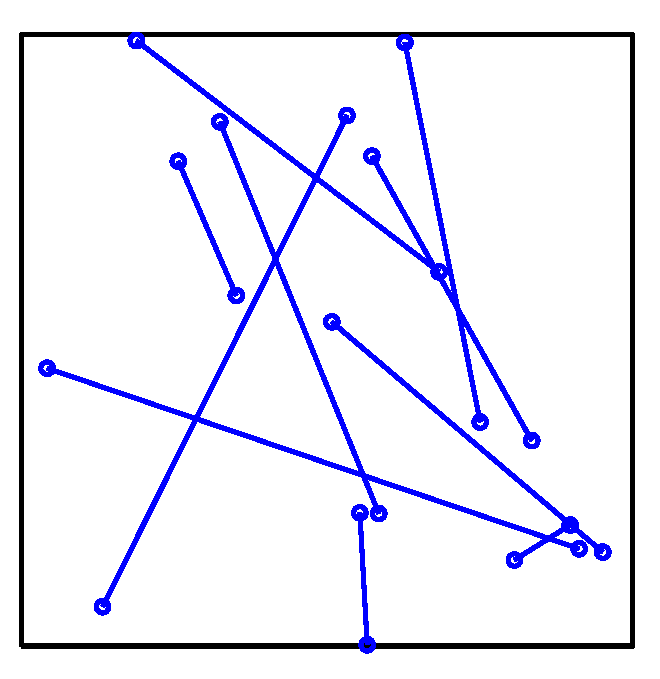
\includegraphics[width=0.3\columnwidth]{../Matlab/Plots/LinePicking_eg_square.eps}} 
       \hspace{0.075\columnwidth}
    \subfloat[\label{fig:square_pdf}PDF.]
       {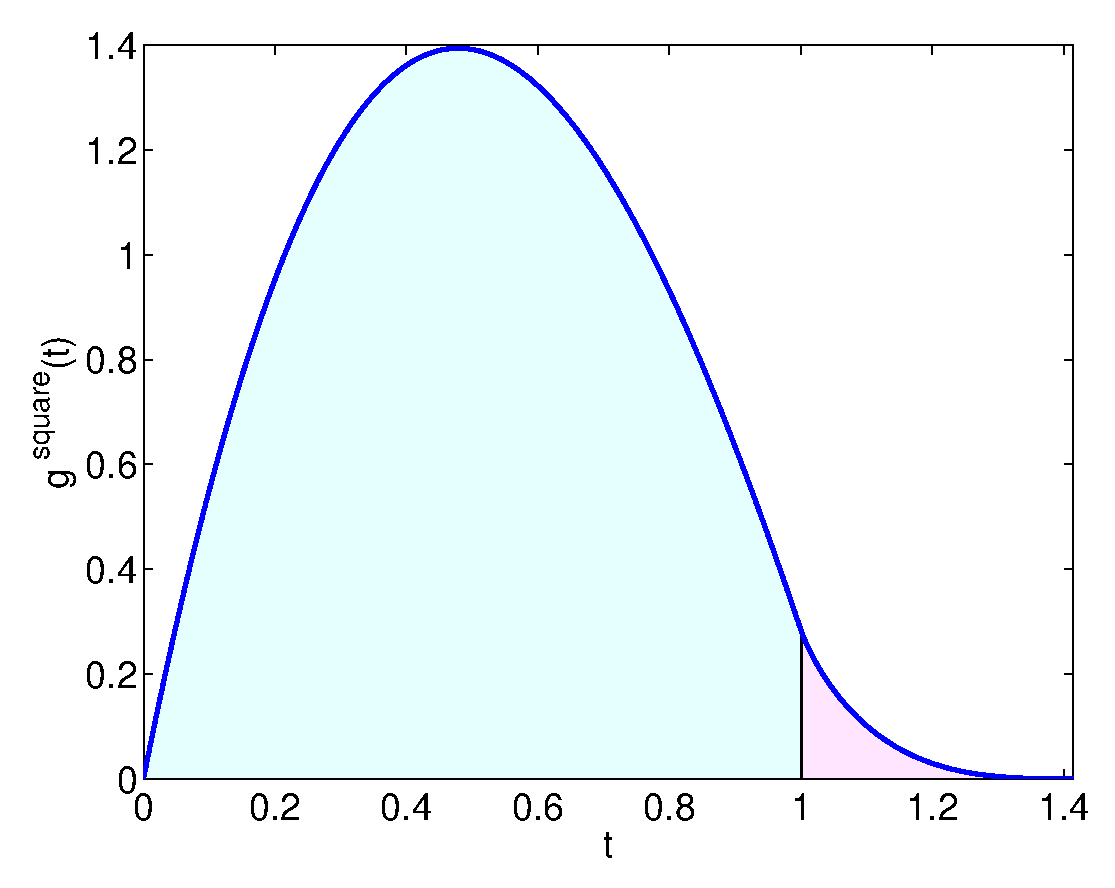
\includegraphics[width=0.5\columnwidth]{../Matlab/Plots/LinePicking_plot_square_pdf.eps}}
    \caption{The unit-square line-picking problem.}
  \end{center} 
\vspace{-4mm}
\end{figure}

\begin{table}[ht]
  \centering
  \begin{tabular}{|r|c|l|}
    \hline
    Statistic & Value & Source \\ 
    \hline
      Support            & $t \in [0, \sqrt{2}]$ & \\
      PDF                & $\displaystyle 
  g^{\rm square}(t) = \left\{ \begin{array}{ll}
      2t (t^2-4t+\pi),
               & \mbox{ for } 0 \leq t \leq 1, \\
      2t \left[4 \sqrt{t^2-1} - (t^2+2-\pi) - 4 \tan^{-1} \left(\sqrt{t^2-1} \right)\right], 
               & \mbox{ for } 1 \leq t \leq \sqrt{2} . \\ 
    \end{array} \right.
                                 $ &
                             \cite{philip:_probab_distr_distan_between_two,weisstein:_squar_line_picking} \\
      CDF                & $\displaystyle
  G^{\rm square}(t) = \left\{ \begin{array}{ll}
      \frac{1}{2} t^4 - \frac{8}{3} t^3 + \pi t^2, 
               & \mbox{ for } 0 \leq t \leq 1, \\
      -\frac{1}{2} t^4 + (\pi-2)t^2 + \frac{1}{3}
                   +\frac{4}{3} \left( 2t^2+1 \right)\sqrt{t^2-1} 
                     & \\
                   \hspace{12mm} - 4 t^2 \tan^{-1} \left(\sqrt{t^2-1} \right),
               & \mbox{ for } 1 \leq t \leq \sqrt{2} . \\ 
    \end{array} \right.
                                 $ & 
                             \cite{weisstein:_squar_line_picking} \\
      $i$th Moment $m_i$ & even moments given in\cite{weisstein:_squar_line_picking} &
                              \cite{weisstein:_squar_line_picking} \\
      Mean               & $\displaystyle \frac{2 \sqrt{2} + 5\sinh^{-1}(1)}{15}
                             = 0.521405433...$ &
                             \cite{weisstein:_squar_line_picking} \\[1.5ex]
      Variance           & $\displaystyle \frac{69 - 4\sqrt{2} -
                             10(2+\sqrt{2}) \sinh^{-1}(1)
                             -25(\sinh^{-1}(1) )^2
                            }{225}
                             = 0.061469...$ &
                             \cite{weisstein:_squar_line_picking} \\[1.5ex]
    \hline
  \end{tabular}
  \caption{Summary of the line-line picking problem for a line of
    length $L$.}
  \label{tab:summary_line}
\end{table}

\subsubsection{PDF}

The PDF for the unit square is given in
\cite{philip:_probab_distr_distan_between_two,weisstein:_squar_line_picking},
but which
\begin{equation}
  \label{eq:square_line}
  g^{\rm square}(t) = \left\{ \begin{array}{ll}
      2t (t^2-4t+\pi), & \mbox{ for } 0 \leq t \leq 1, \\
      2t \left[4 \sqrt{t^2-1} - (t^2+2-\pi) - 4 \tan^{-1} \left(\sqrt{t^2-1} \right)\right], 
               & \mbox{ for } 1 \leq t \leq \sqrt{2} . \\ 
    \end{array} \right.
\end{equation}
% http://mathworld.wolfram.com/SquareLinePicking.html

Generalization to larger squares can be done by scaling (see
Section~\ref{sec:scaling}), or by using the rectangle-line pick1ing
solution (see Section~\ref{sec:rectangle_line}).


 is also a special case of the PDF for the rectangle
\eqref{eqn:rectangle} with $a=b$.

\subsubsection{CDF}
Derived by ...

\begin{equation}
  \label{eq:square_cdf}
  G^{\rm square}(t) = \left\{ \begin{array}{ll}
      \frac{1}{2} t^4 - \frac{8}{3} t^3 + \pi t^2, 
               & \mbox{ for } 0 \leq t \leq 1, \\
      -\frac{1}{2} t^4 + (\pi-2)t^2 + \frac{1}{3}
                   +\frac{4}{3} \left( 2t^2+1 \right)\sqrt{t^2-1} 
                     & \\
                   \hspace{12mm} - 4 t^2 \tan^{-1} \left(\sqrt{t^2-1} \right),
               & \mbox{ for } 1 \leq t \leq \sqrt{2} . \\ 
    \end{array} \right.
\end{equation}

\subsubsection{Moments}



\subsubsection{Related Problems}

A related problem we don't include here (at the moment) is the problem
of choosing two points on two (different) edges of a square.

\url{http://oeis.org/A091506}

D. H. Bailey, J. M. Borwein, V. Kapoor and E. Weisstein, Ten Problems
in Experimental Mathematics

average distance is $(2 + sqrt(2) + 5*ArcSinh[1])/9$

